\documentclass{standalone}

\usepackage[OT1]{fontenc}
\renewcommand*\familydefault{\sfdefault}
\usepackage{helvet,sfmath}
\usepackage{siunitx}

\usepackage{tikz}
\usetikzlibrary{arrows,calc,patterns}
\usepackage{tikz,tkz-euclide}

\usetikzlibrary{decorations.markings}

%% midarrow
\tikzset{
    mid arrow/.style={
        decoration={markings, mark=at position 0.5 with {\arrow{stealth}}},
        postaction={decorate}
    }
}

%% Color
\definecolor{Wave}{RGB}{3, 49, 161}  % #0331A1
\definecolor{M_dipole}{RGB}{0, 127, 189} % #007FBD
\definecolor{J_Current}{RGB}{91, 199, 225} % #5BC7E1
\definecolor{Orange_note}{RGB}{248, 136, 16} % #F88810
\definecolor{P_dipole}{RGB}{201, 1, 161}  % #C901A1
\definecolor{E}{RGB}{113, 11, 121} % #710B79

\begin{document}

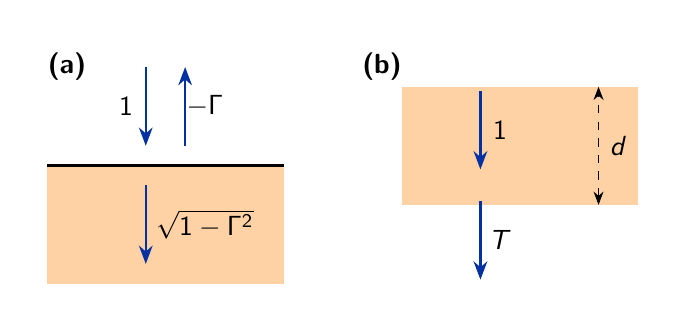
\begin{tikzpicture}[scale=0.5]
    %% Background
    \draw[draw=none] (-8,-3.5) rectangle (8,3.5);

    %% Material
    \draw[draw=none, fill=orange!35] (-7.5,0) rectangle (-1.5,-3);
    \draw[thick] (-7.5,0) to (-1.5,0);

    %% Wave
    \draw[thick, Wave, -Stealth] (-5,2.5) to (-5,0.5);
    \draw[thick, Wave, -Stealth] (-4,0.5) to (-4,2.5);

    \draw[thick, Wave, -Stealth] (-5,-0.5) to (-5,-2.5);

    \draw
    (-5.5, 1.5) node{\(1\)}
    (-3.5, 1.5) node{\(-\Gamma\)}
    (-3.5, -1.5) node{\(\sqrt{1 - \Gamma^2}\)}
    (-7,2.5) node{\textbf{(a)}}
    ;

    
    %% Material
    \draw[draw=none, fill=orange!35] (1.5,-1) rectangle (7.5,2);

    \draw[dashed, Stealth-Stealth] (6.5,-1) to (6.5,2);
    \draw (7,0.5) node{\(d\)};

    %% Wave
    \draw[thick, Wave, -Stealth] (3.5,1.9) to (3.5,-0.1);
    \draw[thick, Wave, -Stealth] (3.5,-0.9) to (3.5,-2.9);

    \draw
    (4,0.9) node{\(1\)}
    (4,-1.9) node{\(T\)}
    (1,2.5) node{\textbf{(b)}}
    ;
    
    
    
\end{tikzpicture}

\end{document}